
\chapter{Volatilities of Neural Models}
\label{chapter:research-05}


\section{Introduction and research questions}

In the previous chapters, we first investigated how to enhance the use of context to address some of the shortcomings of neural translation models. 
%Challenges for neural translation models, when sufficient data is not available, include understanding rare words \citep{W18-2712} and domain mismatch between training and testing \citep{koehn2017six,W18-2709}.
Then in Chapter~\ref{chapter:research-04}, we showed that the translation of idiomatic phrases is challenging for the current NMT models. 
We saw that the scope of the observed context was not sufficient to infer the meaning of idioms.
Based on these findings, in this chapter, we continue examining the following question:

\paragraph{Research Question 3:} \acl{rq:vol} 

\medskip

 \noindent 
 While the lack of suitable context exposes shortcomings in current models, we extend our research in this chapter to situations where appropriate data \textit{is} available. 
We first look into the robustness of current translation models.
Namely, we investigate what is the effect of small perturbations of the source sentence on the translation.
Observing that in some cases translations change unexpectedly with these small perturbations, 
we study whether and to what extent it can be replicated and quantified with automatically modified test data. 
Concretely we ask:
 
\begin{enumerate}[label=\textbf{RQ3.\arabic* },wide = 0pt, leftmargin=2em]
\setlength\itemsep{1em}
 \setcounter{enumi}{2}
\item \acl{rq:vol1}

\medskip

\noindent To answer this question, we locally modify sentence pairs in the test set and identify examples where a trivial modification in the source sentence causes an `unexpected change' in the translation.
These modifications are generated conservatively to avoid insertion of any noise or rare words in the data (Section~\ref{secsentvar}). 
Our goal is not to \textit{fool} the NMT models, but instead, to identify common cases where the models exhibit unexpected behaviour and in the worst cases result in incorrect translations. 
We identify these unexpected and erroneous changes in the translation output as a sign of an underlying \textit{volatility} of NMT models. 

\item \acl{rq:vol2}

\medskip

\noindent We investigate to what extent two current state-of-the-art NMT models are robust against changes in the input during inference.
We observe that our modifications expose volatilities of both RNN and Transformer translation models in $26\%$ and $19\%$ of sentence variations, respectively.
Our findings show how vulnerable current NMT models are to trivial linguistic variations, putting into question the generalization abilities of these models. 
%This volatile behavior of translating extremely similar sentences in surprisingly different ways highlights the underlying generalization problem of current NMT models. 

\end{enumerate}

\paragraph{Organization.} The chapter is organized as follows: 
Section~\ref{isitanothernoise} discusses prior works on the impact of noise on the performance of machine translation.
In Section~\ref{secvol}, we provide an example of unexpected behaviour of NMT models and discuss how it is different from the unexpected behaviour when encountering noise in the input text. 
In Section~\ref{secsentvar}, we introduce our sentence variation generation approach and provide details on the experimental settings.
Section~\ref{secvolassess} proposes various metrics to identify and quantify these unexpected changes and provides experimental results on a translation task.
Finally, we discuss the conclusions and implications of this work in Section~\ref{secvolconc}. 

\section{Noisy text translation} \label{isitanothernoise}

Recently, several approaches investigated NMT models when encountering noisy input and how \textit{worst-case examples} of noisy input can `break' state-of-the-art NMT models \citep{D18-1050}. 
Noisy input text can cause mistranslations in most translation systems, and there has been growing research interest in studying the behaviour of translation systems when encountering noisy input \citep{li-EtAl:2019:WMT1}.

\citet{DBLP:journals/corr/abs-1711-02173} show that character-level noise in the input %, for instance swapping random letters of a word, 
leads to poor translation performance.
They propose to swap or randomize letters in a word in the input sentence. For instance, they change the word `\textit{noise}' in the source sentence into `\textit{iones}'.
\citet{halluc} randomly insert words in different positions in the source sentence and observe that in some cases the translations are completely unrelated to the input. 
\citet{D18-1050} propose a benchmark data set for translation of noisy input sentences, consisting of noisy, user-generated comments on Reddit.
The types of noisy input text they observe include spelling or typographical errors, word omission/insertion/repetition, and grammatical errors.


\section{Volatility in machine translation} \label{secvol}

In the discussed works in Section~\ref{isitanothernoise}, the focus of the research is on studying how the translation systems are not robust when handling noisy input text. In these approaches, the input sentences are semantically or syntactically incorrect which leads to mistranslations. 
However, in this chapter, our focus is on input text that does \textit{not} contain any types of noise. We modify input sentences in a way that the outcomes are still syntactically and semantically correct. 
We investigate how translation systems exhibit volatile behaviour in translating sentences that are extremely similar and only differ in one word without any noise injection.
While it is to some extent expected that the performance of NMT models that are trained on predominantly clean but tested on noisy data deteriorates, other changes are more unexpected.


\begin{table}[ht]
\centering
\caption{Insertion of the German word \textit{`sehr'} (English: \textit{`very'}) in different positions in the source sentence results in substantially different translations. Note that all source sentences are syntactically correct and semantically plausible. We use a Transformer model trained on WMT data with 6 encoder and decoder layers and 8 attention heads. $^\dagger$ indicates the original sentence from WMT 2017. \label{first}}
%\setlength\tabcolsep{5pt} % default value: 6pt
\begin{tabularx}{0.7\textwidth}{lll}
%Source & Translation \\ 
\multicolumn{3}{l}{\textcolor{mygray}{Source:} \textit{Ich bin \underline{\ \ \ \ \ \ }\ \raisebox{-1.5ex}{\tiny{\fbox{$1$}}} \textbf{erleichtert} und \underline{\ \ \ \ \ \ }\ \raisebox{-1.5ex}{\tiny{\fbox{$2$}}} bescheiden.}}\\
%\multicolumn{3}{l}{\textcolor{mygray}{Reference:} \textit{I am relieved and humble.}} \\
\hline
\\[-0.5ex]
\fbox{$1$} &  \fbox{$2$} & \textcolor{mygray}{NMT output} \\
\hline
%\multicolumn{4}{l}{} \\ % & I am relieved and very modest. \\
%\multicolumn{2}{l}{ I am relieved and \textbf{very} modest.} \\
  $\phi$ & $\phi$   & I am \underline{easier} and modest.  \\ 
  $\phi$ & \textit{sehr} $ ^{\dagger}$&  I am \textbf{relieved} and very modest. \\ 
%Ich bin erleichtert und bescheiden. & I am easier and modest. \\
  \textit{sehr} & $\phi$ & I am {very} much \underline{easier} and modest.  \\ 
%Ich bin sehr erleichtert und bescheiden. & I am very much easier and modest. \\
  \textit{sehr} & \textit{sehr} & I am {very} \underline{easy} and {very} modest.   \\ 
%Ich bin sehr erleichtert und sehr bescheiden. & I am very easy and very modest. \\
\\
&& \textcolor{mygray}{Reference}\\
\hline
 $\phi$ & $\phi$   & \textit{I am relieved and humble.}\\
  \textit{sehr} & \textit{sehr} & \textit{I am very relieved and very humble.}   \\ 
\end{tabularx}
\end{table}

In this chapter, we explore unexpected and erroneous changes in the output of NMT models.
Consider the simple example in Table~\ref{first} where the Transformer model 
is used to translate very similar sentences.
Surprisingly, we observe that by simply altering one word in the source sentence---inserting the German word \textit{`sehr'} (English: \textit{`very'})---an unrelated change occurs in the translation.
In principle, an NMT model that generates the translation of the word \textit{`erleichtert'} (English: \textit{`relieved'}) in one context, should also be able to generalize and translate it correctly in a very similar context.
Note that there are no infrequent words in the source sentence and after each modification, the input is still syntactically correct and semantically plausible.
We call a model \textit{volatile} if it displays inconsistent behaviour across similar input sentences during inference. 


\section{Variation generation}   \label{secsentvar}

While there are various ways to automatically modify sentences, we are interested in simple semantic and syntactic modifications. % in changing the meaning of the sentence.
These trivial linguistic variations should have almost no effect on the translation of the rest of the sentence.

%\subsection{Classes of Modifications}

%The modifications with the least variations in meaning result in very similar sentences to the original sentence. 
%We are interested in trivial linguistic variations with almost no effect on the translation of the rest of the sentence.
We define a set of rules to slightly modify the source and target sentences in the test data and keep the sentences syntactically correct and semantically plausible. 

%The rules take the form $r = (w_i \rightarrow w_j)$, where the word $w_i$ in the original source sentence is replaced by the word $w_j$.
%Depending on the rule, we also modify the corresponding target sentence. 

\begin{itemize}%[noitemsep,nolistsep]
\item \textbf{Delete}: A conservative approach to modifying a sentence automatically without breaking its grammaticality is to remove adverbs. 
We identify a list of the 50 most frequent adverbs in English and their translations in German.\footnote{Here, we use the \url{dict.cc} online dictionary.}
For every sentence in the WMT test sets, if we find a sentence pair containing both a word and its translation from this list, we remove both words and create a new sentence pair. 
\item \textbf{Insert}: Randomly inserting words in a sentence has a high chance of producing a syntactically incorrect sentence.
To ensure that sentences remain grammatical and semantically plausible after modification, we define a bidirectional n-gram probability for inserting new words as follows:
\begin{equation}
P(w_3 \mid w_1 w_2 w_4 w_5) = \frac{C(w_1 w_2 w_3 w_4 w_5)}{\sum_j C(w_1 w_2 w_j w_4 w_5)}
\end{equation}
$w_3$ is inserted in the middle of the phrase $w_1 w_2 w_4 w_5$, if the conditional probability is greater than a predefined threshold.  
The probabilities are computed on the WMT data.
This simple approach, instead of using a more complex language model, serves our purposes since we are interested in inserting very common words that are already captured by the n-grams in the training data.

\item \textbf{Substitute number}: Another simple yet effective approach to safely modifying sentences % ensuring that we do not inject noise into the test set 
is to substitute numbers with other numbers.
In this approach, we select every sentence pair from the test sets that contain a number and substitute the number $i$ in both source and target sentences with $i+k$ where $1 \leq k \leq 5$.
We choose a small range for change so that the sentences are still semantically correct for the most part and result in a few implausible sentences.
%The new test set is augmented with all of the new sentence pairs.
\item \textbf{Substitute gender}: Finally, a local modification  
is to change the gender of the pronoun in the sentences. 
The goal of this modification is to investigate the existence and severity of gender bias in our models.
This is inspired by recent approaches that have shown that NMT models learn social stereotypes such as gender bias from training data \citep{escude-font-costa-jussa-2019-equalizing,stanovsky-etal-2019-evaluating}.  
\end{itemize}

Note that in a minority of cases, these procedures can lead to semantically incorrect sentences.
For instance, by substituting numbers we can potentially generate sentences such as \textit{''She was born on October 34th``}. 
While this can cause problems for a reasoning task, it barely affects the translation task, as long as the modifications are consistent on the source and target side. 


Table~\ref{examplesofpert} shows examples of generated variations. %from each class of modification.
We emphasize that only modifications with local consequences have been selected and we intentionally ignore cases such as \textit{negation} which can result in wider structural changes in the translation of the sentence.

\begin{table}[ht]
\begin{center}\small
\setlength\tabcolsep{4pt} % default value: 6pt
\caption{\label{examplesofpert} Examples of different variations from WMT. [$w_i$\textbackslash$w_j$] indicates that $w_i$ in the original sentence is replaced by $w_j$. ${\phi}$ is the empty string.}
\begin{tabularx}{0.9\columnwidth}{lX}
\toprule
\bf Modification & \bf Sentence variations\\
\midrule
\textit{Delete} &  Some 500 years after the Reformation, Rome  \textbf{[now\textbackslash$\pmb{\phi}$]} has a Martin Luther Square. \\
\textit{Insert} & I loved Amy and she is  \textbf{[$\pmb{\phi}$\textbackslash also]} the only person who ever loved me.  \\
%according to press reports , the party have threatened Trump with removing financial support for his election campaign if he is unable to do any better in the \textbf{opinion} polls . \\
 %\midrule
%\texttt{del} & But despite the smiles for the cameras, few here are convinced-especially [\textbf{now} / $\pmb{\phi}$], just before parliamentary elections.\\
\textit{Subs number} & I'm very pleased for it to have happened at Newmarket because this is where I landed \textbf{[30\textbackslash31]} years ago. \\
\textit{Subs gender} & \textbf{[He\textbackslash She]} received considerable appreciation and praise for this. \\
%but despite the smiles for the cameras , few here are convinced - especially , just before parliamentary elections .\\
\bottomrule
\end{tabularx}
\end{center}
\end{table} 

 
%In the next section we discuss the results and analyze volatilities of the NMT models.
We generate 10K sentence variations by applying these modifications to all sentence pairs in WMT test sets 2013--2018 \citep{bojar-EtAl:2018:WMT1}. %to generate variations of the same sentences. %and for each class of modification different number of new sentences are generated.% (presented in Table~\ref{counts}).
%Note that we generate different number of new sentences for different modification classes due to the nature of the modifications and the available words in the sentences.
% from WMT test sets.
We use RNN and Transformer models to translate sentences and their variations.

\subsection{Experimental setup}

In the translation experiments, we use the standard English$\leftrightarrow$German WMT-2017 training data % and report results on newstest 2013-2018 
\citep{bojar-EtAl:2018:WMT1}.
We perform NMT experiments with two different architectures as described in Sections~\ref{RNN} and~\ref{TRNN}: RNN \citep{luong:2015:EMNLP} and Transformer \citep{vaswani2017attention}.
We preprocess the training data with Byte-Pair Encoding (BPE) using 32K merge operations \citep{sennrich-haddow-birch:2016:P16-12}. %to segment words into subword units for both languages.
Table~\ref{bleus} shows the case-sensitive BLEU scores as calculated by \texttt{multi-bleu.perl}. %on WMT test sets 2016 and 2017.

\begin{table}[ht]
\center
\setlength\tabcolsep{3pt} % default value: 6pt
\caption{\label{bleus} BLEU scores of different baseline models on the WMT news data for translation of German$\leftrightarrow$English.}
\begin{tabular}{@{\extracolsep{4pt}}lcccccc@{}}
\toprule
 & \multicolumn{3}{c}{\bf De-En} &  \multicolumn{3}{c}{\bf En-De} \\ \cline{2-4}  \cline{5-7}   
 &   WMT16 &  WMT17 &  WMT18  &  WMT16 &  WMT17  &  WMT18  \\ \midrule
RNN & 32.5 & 28.2 &35.2 & 28.1  & 22.4 & 34.6 \\ 
Transformer & 36.2 & 32.1 & 40.1 & 33.4 & 27.9& 39.8  \\
\bottomrule
\end{tabular}
\end{table}


\paragraph{RNN} We use a 2-layer bidirectional attention-based LSTM model implemented in OpenNMT \citep{2017opennmt} trained with an embedding size of 512, hidden dimension size of 1024, and batch size of 64 sentences. We use Adam \citep{kingma2014adam} for optimization.

\paragraph{Transformer} We also experiment with the Transformer model \citep{vaswani2017attention} implemented in OpenNMT. We train a model with 6 layers, the hidden size is set to 512, and the filter size set to 2048. The multi-head attention has 8 attention heads. We use Adam \citep{kingma2014adam} for optimization. All parameters are set based on the suggestions by \citet{2017opennmt} to replicate the results of the original paper.


\section{Unexpected and erroneous changes} \label{secvolassess}

The modifications described above generate sentences that are extremely similar %to the original sentences 
and hence are expected to have a very similar difficulty of translation. 
First, we evaluate the NMT models on how robust and consistent they are in translating these sentence variations rather than their absolute quality.
Next, we perform manual evaluation on the translation outputs to assess the impact of unexpected changes on translation quality.  
%To this end, we provide a more detailed analysis on unexpected changes in translations here.


\subsection{Deviations from original translation}\label{ctsec}

The variations are aimed to have minimal effect on changing the meaning of the sentences. 
Hence, major changes in the translations of these variations can be an indication of volatility in the model.
To assess whether the proposed sentence variations result in major changes in the translations, we measure changes in the translations of sentence variations with Levenshtein distance \citep{levenshtein1966binary}. %and \textit{span of change}.
%Specifically, Levenshtein distance measures the edit distance between the two translations. %while span of change indicates the spread of changes in the sentence.
We also use the first and last positions of change in the translations, which represents the span of changes.

\begin{figure*}[tbh!]
\centering
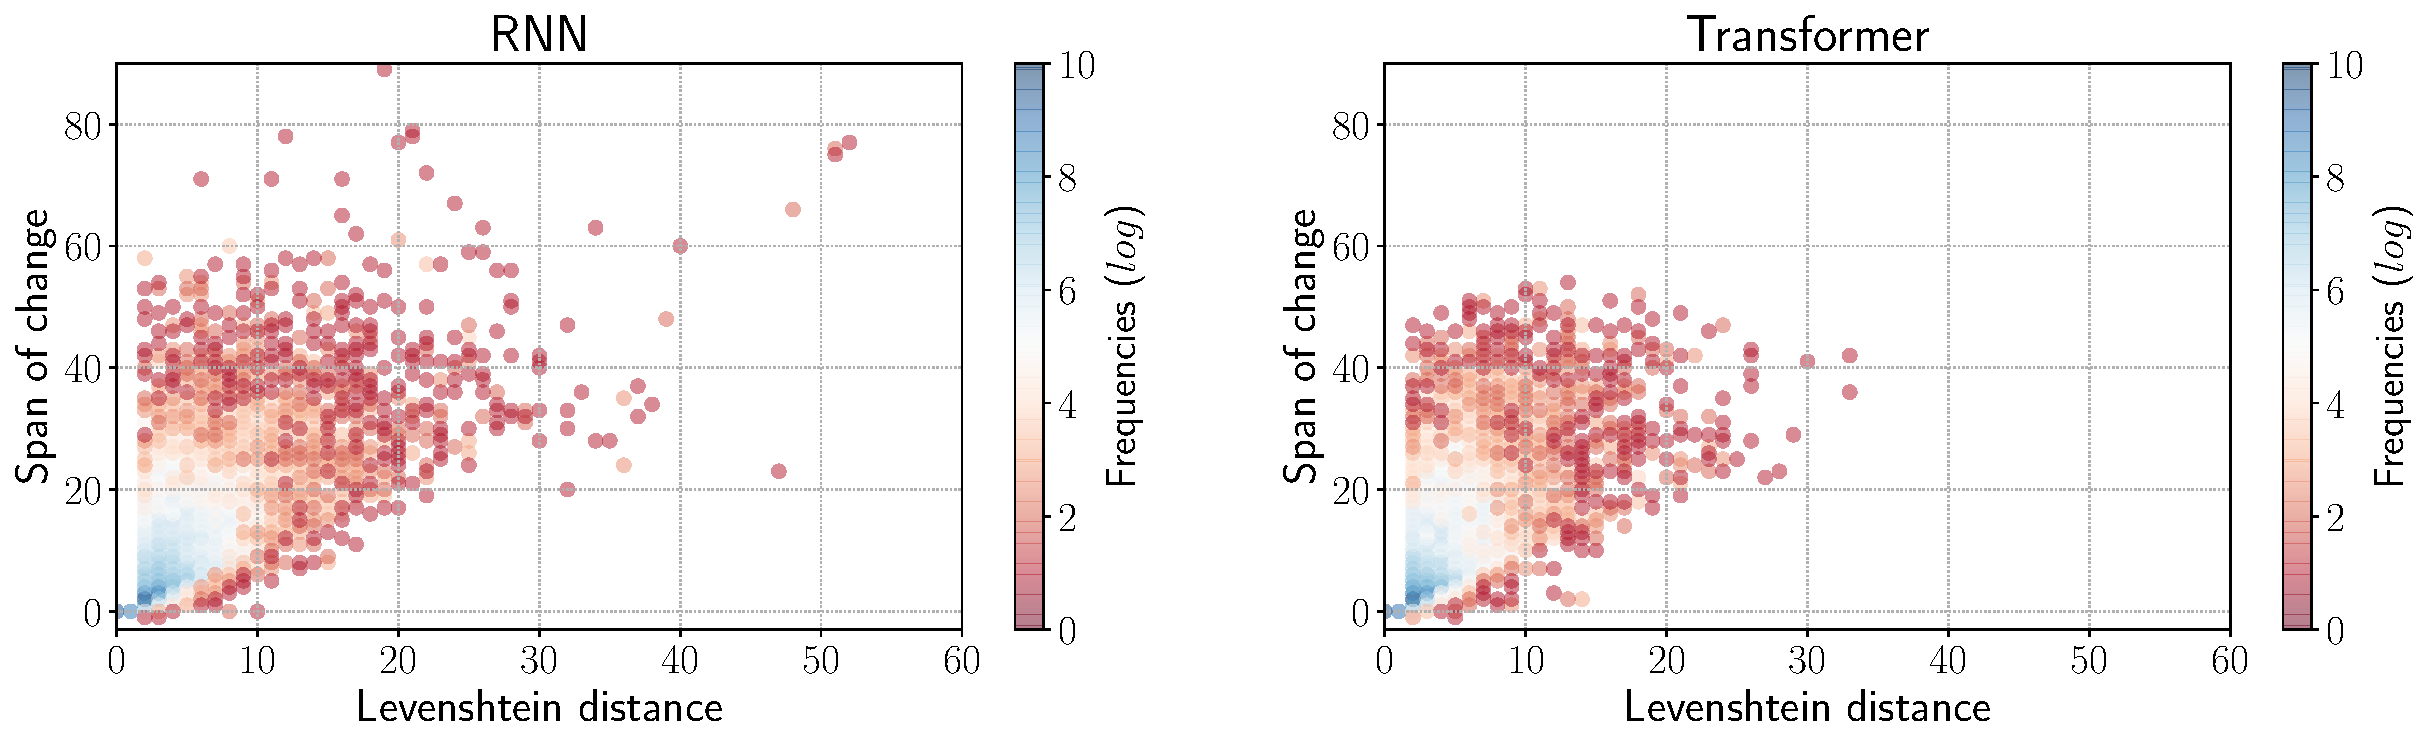
\includegraphics[width=\textwidth]{07-research-05/figs/plot2.pdf}
\caption{\textit{Levenshtein distance} and \textit{span of change} between translations of sentence variations for RNN and Transformer. %With extremely similar sentence variations, we observe major differences between the translations for a surprising number of sentences.
The majority of sentence variations fall into the category of \textit{minor} changes between translations (blue area). However, a surprising number of cases have significant changes (red area). RNN exhibits a slightly more unstable pattern i.e., sentence variations with large edit differences and large spans of change.
}
\label{fig1}
\end{figure*}

Ideally, with our simple modifications, we expect a value of zero for the span of change and a value of at most 2 for the Levenshtein distance for a translation pair.
This indicates that there is only one token difference between the translation of the original sentence and the modified sentence. 

We define two types of changes based on these measures: \textit{minor} and \textit{major}.
We choose the threshold to distinguish between minor and major changes conservatively to allow for more variations in the translations.
The change in translations is empirically considered \textit{major} if both metrics are greater than 10, and \textit{minor} if both are less than 10. 
Note that edit distances and spans are based on BPE subword units.

With two very similar source sentences, we expect the Levenshtein distance and span of change between translations of these sentences to be small.
%\todo{This means that unexpected change is just the same as major??? So why bother with the extra terminolog?} 
Figure~\ref{fig1} shows the results for the RNN and Transformer model. 
%Surprisingly, we observe that our local modifications results in significant changes in a number of sentences. 
While the majority of sentence variations have minor changes, %after the modification, % i.e., small Levenshtein distance and span of change, 
a substantial number of sentences, $18\%$ of RNN and $13\%$ of Transformer translations, result in translations with major differences. % major changes in the translations % in the sentence variations.
This is a surprising indication of volatility since these trivial modifications, in principle, should only result in minor and local changes in the translations. 



\begin{table}[htb!]
\centering
\caption{An example of the generated variations of an English sentence and different sentence-level metrics for the translation of each variation. We compute the oscillation range for each sentence in the test data. \label{oscmetexams}}
\begin{tabularx}{.97\columnwidth}{ll}
%Source & Translation \\ 
\toprule
Source: & \textit{Mr Ivanov took up the post in December {$\spadesuit$}.} \\
Reference: & \textit{Ivanov nahm den Posten im Dezember {$\spadesuit$} an.} \\
\hline
\\[-0.5ex]
{$\spadesuit$}  & \textcolor{mygray}{NMT output} \\
\hline
  \textit{2012} & Herr Ivanov hat den Beitrag im Dezember 2012 {\"u}bernommen.  \\
  &  \textcolor{mygray}{\textit{bleu=22.78 meteor=60.54 ter=36.36 LengthRatio=109.09}} \\
  \textit{2013} &  Herr Ivanov nahm den Beitrag im Dezember 2013 auf.  \\
  &  \textcolor{mygray}{\textit{bleu=43.67, meteor=66.89, ter=27.27, LengthRatio=109.09}} \\
  \textit{2014} &  Herr Ivanov nahm den Beitrag im Dezember 2014 auf. \\
  &  \textcolor{mygray}{\textit{bleu=43.67, meteor=66.89, ter=27.27, LengthRatio=109.09}} \\
  \hline % \\[-2ex]
{Oscillation range:} & \textit{bleu=20.9, meteor=6.4, ter=9.1, LengthRatio=0} \\
\bottomrule
\end{tabularx}
\end{table}

\subsection{Oscillations of variation in translations}

In this section, we look into various sentence-level metrics to further analyze the observed behaviour. 
In particular, we focus on the \textit{substitute numbers} modification since with this modification, we can easily generate numerous variations of the same sentence. % is easy and noise-proof. 
Having a high number of variations for each sentence gives us the opportunity of observing oscillations of various string matching metrics. 

We use sentence-level BLEU, METEOR \citep{denkowski-lavie-2011-meteor}, TER \citep{Snover06astudy}, and LengthRatio to quantify changes in the translations.
LengthRatio represents the translation length over reference length as a percentage.
For a given source sentence, we define the \textit{oscillation range} as changes in the sentence-level metric for
 the translations of all variations of the sentence (see Table~\ref{oscmetexams} for an example). 


\begin{figure*}[htb!]
\centering
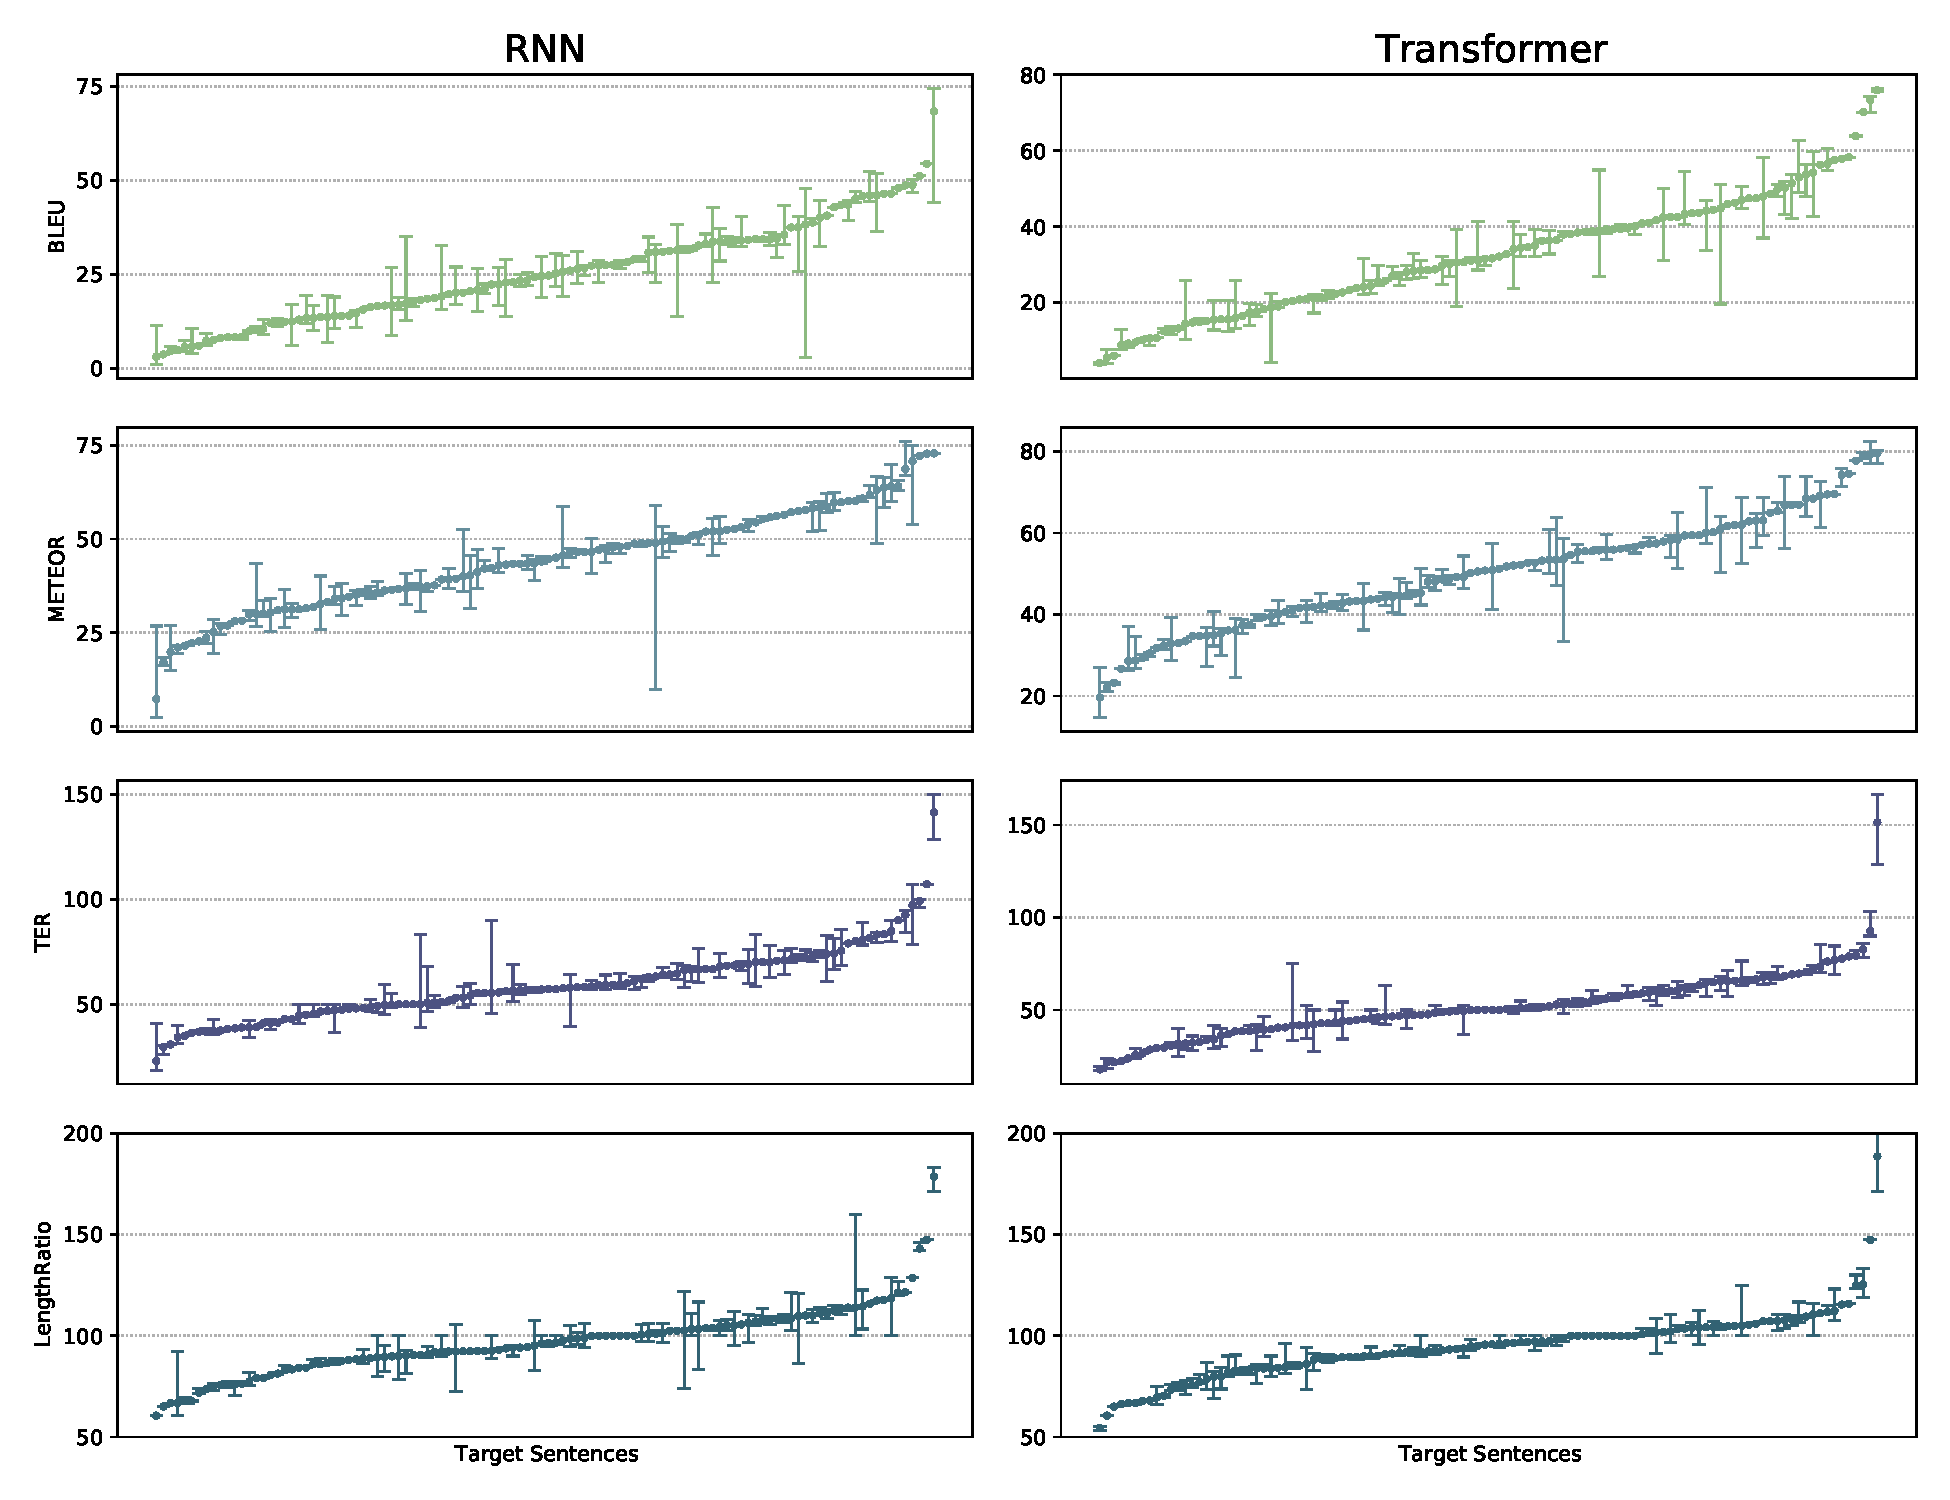
\includegraphics[width=1\textwidth]{07-research-05/figs/oscs.pdf}
\caption{Oscillations of various sentence-level attributes for randomly sampled sentences from our test data and their \textit{substitute number} variations. 
The data points are the mean values for all variations of each sentence, and the error bars indicate the range of oscillation of the metrics. The x-axis represents test sentence instances, sorted based on the corresponding metric. 
Ideally, each data point should have zero oscillation. }
\label{figosc}
\end{figure*}

\begin{table}[ht]
\center
\small
%\setlength\tabcolsep{4.5pt} % default value: 6pt
\caption{\label{oscstats} Mean oscillations for \textit{substitute number} variations. In theory, the variations should result in zero oscillations for every metric.}
\begin{tabularx}{0.63\columnwidth}{lcccc}
\toprule
% & \multicolumn{3}{c}{\bf DE-EN} &  \multicolumn{3}{|c}{\bf EN-DE} \\
& \bf BLEU & \bf METEOR & \bf TER & \bf LengthRatio \\
\midrule
RNN & 4.0 & 3.8& 5.2 & 5.3 \\ 
Transformer & 3.8 & 3.3 & 4.2 & 3.4  \\
\bottomrule
\end{tabularx}
\end{table}


While sentence-level metrics are not reliable indicators of translation quality, they do capture fluctuations in translations.  
With the variations we introduced, in theory, there should be no fluctuations in the translations. 
Figure~\ref{figosc} and Table~\ref{oscstats} provide the results. 
We observe that even though these sentence variations differ by only one number, there are many cases where an insignificant change in the sentence results in unexpectedly large oscillations. Both RNN and Transformer exhibit this behaviour to a certain extent. 


\subsection{The effect of volatility on translation quality}

While edit distances, spans of change, and oscillation in variations provide some indication of volatility, they do not capture all aspects of this unexpected behaviour. 
It is also not entirely clear what effect these unexpected changes have on translation quality.
To further investigate this, we also perform two manual evaluations by eight fellow PhD students working on information and language processing systems.
The native language of the annotators consists of English, Dutch, and Chinese. 
All non-native annotators use English as a second language.
Our manual evaluation does not require familiarity with the German language.

In the first evaluation, we provide annotators with a pair of sentence variations and their corresponding translations
%the translation pairs of sentence variations 
and ask them to identify the differences between the two sentence pairs.
In the second evaluation, we additionally provide the source sentences and reference translations and ask the annotators to rank the sentence variations based on the translation quality similar to \citet{bojar-EtAl:2016:WMT1}.
In total, the annotators evaluated 400 randomly selected sentence quadruplets. 
 
 \begin{table*}[htb!]
\centering \small
\caption{Definitions of different labels of changes and examples for each category. The annotators identified these differences between the translations. \label{guidelinestab} }
\begin{tabularx}{0.95\columnwidth}{lXX}
\bf Label & \bf Definition & \bf Example  \\ \toprule
\texttt{Word form} & One or more words are different in form but belong to the same lexeme.   & \textit{observe} $\rightarrow$ \textit{observation} \\
\texttt{Reordered} & One or more words are reordered in the translation sentence.   & \textit{he said go}  $\rightarrow$ \textit{go, he said} \\
\texttt{Paraphrased} & One word is replaced with a synonym or a section of the sentence is paraphrased. & \textit{first six months} $\rightarrow$ \textit{first half of the year} \\
\texttt{Add/Remove} & One or more words are added or dropped from the translation sentence. & \textit{will participate} $\rightarrow$  \textit{will also participate}   \\
\texttt{Other}  & Other changes in the translation sentence.  & \textit{were torn through} $\rightarrow$  \textit{have been bypassed}   \\
\end{tabularx}
\end{table*}
%
\begin{table*}[htbp!]
 \begin{small}
\begin{center}
\setlength\tabcolsep{4pt} % default value: 6pt
\caption{\label{man}  A random sample of sentences from the WMT test sets and our proposed variations shown with `unexpected change' annotations ($\Delta Translation$). The cases where the unexpected change leads to a change in translation quality are marked in column $\Delta Quality$. [$w_i$\textbackslash$w_j$] indicates that $w_i$ in the original sentence is replaced by $w_j$. $S$ is the original and modified source sentence, $R$ is the original and modified reference translation, $T$ is the translation of the original sentence, and $T_m$ is the translation of the modified sentence. Differences in translations related to annotations are underlined.}
\begin{tabularx}{\textwidth}{lX}
\toprule
${S}$ &   Coes letztes Buch "Chop Suey" handelte von der chinesischen K{\"u}che in den USA, w{\"a}hrend Ziegelman in ihrem Buch "\textbf{[97\textbackslash 101]} Orchard" {\"u}ber das Leben in einem Wohnhaus an der Lower East Side aus der Lebensmittelperspektive erz{\"a}hlt.  \\
${R}$ & Mr. Coe's last book, "Chop Suey," was about Chinese cuisine in America, while Ms. Ziegelman told the story of life in a Lower East Side tenement through food in her book "\textbf{[97\textbackslash 101]} Orchard."  \\ 
%\midrule
${T}$ &   Coes\underline{'s} last book, "Chop Suey," was about Chinese cuisine in the \underline{US}, while Ziegelman, \underline{in her book "97 Orchard" talks about} living in a lower East Side.  \\
${T_m}$ &  Coes last book "Chop Suey" was about Chinese cuisine in the \underline{United States}, while Ziegelman \underline{writes in her book "101 Orchard" about} living in a lower East Side. \\ %&&\cmark&\cmark&&& \xmark \\
%\hdashline
  \rowcolor{tablegray}   \multicolumn {2}{l}{\textcolor{mygray}{\texttt{$\Delta Translation$: [reordered] [paraphrased] |  $\Delta Quality$: No }}}  \\
  \midrule
 ${S}$ &  Man h{\"a}lt \textbf{[bereits\textbackslash$\pmb{\phi}$]} Ausschau nach Parkbank, Hund und Fu{\ss}ball spielenden Jungs und M{\"a}dels. \\
$R$ & You are \textbf{[already\textbackslash$\pmb{\phi}$]} on the lookout for a park bench, a dog, and boys and girls playing football. \\
%\midrule
${T}$ & \underline{We are} already \underline{looking} for Parkbank, dog and football playing boys and girls.  \\
${T_m}$& \underline{Look} for Parkbank, dog and football playing boys and girls. \\ %&\cmark&&&\cmark& & \cmark \\
%\hdashline
  \rowcolor{tablegray}   \multicolumn {2}{l}{\textcolor{mygray}{\texttt{$\Delta Translation$: [word form] [add/remove] | $\Delta Quality$: Yes }}}  \\
  \midrule
%$\Delta$ & \multicolumn {1}{l}{\textcolor{mygray}{\texttt{[word form] [add/remove]}}}\\
%\midrule
${S}$ 	& Bei einem Unfall eines Reisebusses mit \textbf{[43\textbackslash 45]} Senioren als Fahrg{\"a}sten sind am Donnerstag in Krummh{\"o}rn (Landkreis Aurich) acht Menschen verletzt worden.  \\
$R$ & On Thursday, an accident involving a coach carrying \textbf{[43\textbackslash 45]} elderly people in Krummh{\"o}rn (district of Aurich) led to eight people being injured. \\
%\midrule
${T}$  &	In the event of an accident involving \underline{a coach with 43 senior citizens} as \underline{passengers}, eight people were injured on Thursday in \underline{Krummaudin (County Aurich)}.  \\
${T_m}$   &	In the event of an accident involving \underline{a 45-year-old coach} as a \underline{passenger}, eight people were injured on Thursday in  \underline{the district of Aurich}. \\% &\cmark&&&\cmark& \cmark &\cmark\\
%\hdashline
%$\Delta$ & \multicolumn {1}{l}{ \textcolor{mygray}{\texttt{[word form] [add/remove] [other]}}}\\
  \rowcolor{tablegray} \multicolumn {2}{l}{\textcolor{mygray}{\texttt{$\Delta Translation$: [word form] [add/remove] [other] | $\Delta Quality$: Yes }}}  \\
\midrule
${S}$  &  Es ist ein anstrengendes Pensum, aber die Dorfmusiker helfen \textbf{[normalerweise\textbackslash$\pmb{\phi}$]}, das Team motiviert zu halten.  \\	
 $R$ & It's a backbreaking pace, but village musicians \textbf{[usually\textbackslash$\pmb{\phi}$]} help keep the team motivated.    \\
% \midrule
${T}$  & It\underline{'s} a \underline{demanding child}, but the village \underline{musicians} usually \underline{help} keep the team motivated.  \\
${T_m}$  & It \underline{is} a \underline{hard-to-use}, but the village \underline{musician} \underline{helps to} keep the team motivated.	\\ %	&\cmark&&& & \cmark&\cmark \\	
%\hdashline
%$\Delta$ & \multicolumn {1}{l}{ \textcolor{mygray}{\texttt{[word form] [other]}}}\\
  \rowcolor{tablegray}   \multicolumn {2}{l}{\textcolor{mygray}{\texttt{$\Delta Translation$: [word form] [other] | $\Delta Quality$: Yes }}}  \\
\bottomrule
\end{tabularx}
 \end{center}
%}
 %\end{center}
 \end{small}
\end{table*}
%
%
  \begin{figure*}[htb!]
\centering
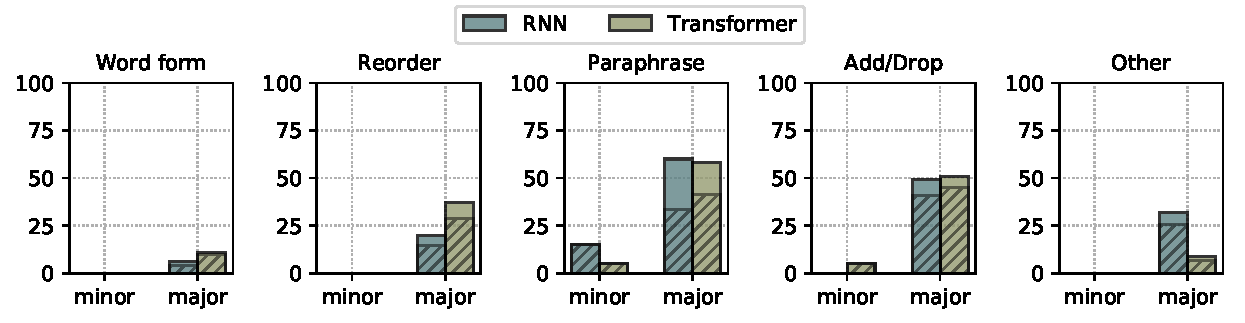
\includegraphics[width=1\textwidth]{07-research-05/figs/plot3.pdf}
\caption{Categories of unexpected changes in the translation of sentence variations as provided by annotators. The percentage of sentence variations with \textit{minor} and \textit{major} edit differences, as defined in~\ref{ctsec}, are shown separately. The hatched pattern indicates the ratio of sentence variations for which the translation quality changes.} %for different sentence variations.}
%Levenshtein distance between translations of sentences before and after modification grouped in 3 buckets. Hatched pattern is the ratio of sentence pairs in each bucket with more than 10 unigram differences.} %en-de.
\label{fig2}
\end{figure*}
%

Table~\ref{guidelinestab} shows the identified categories of changes from annotators' labels.  
The main types of unexpected changes identified by the annotators are a `change of word form', e.g., verb tense, `reordering of phrases', `paraphrasing' parts of the sentence, and an `other' category, e.g., preposition.  
A sentence pair can have multiple labels based on the types of changes. 
Table~\ref{man} provides examples from the test data. %of the types of changes. % in each sentence variation. 
%Note that we are interested in \textit{unexpected} changes and ignore the changes that are a direct consequence of the modifications.

Statistics for each category of unexpected change are shown in Figure~\ref{fig2}.
Our first observation is that, as to be expected, there are very few `unexpected changes' when two variations lead to translations with \textit{minor} differences.
Interestingly, the vast majority of changes are due to paraphrasing and adding or dropping of words.
Comparing the performance of the RNN and Transformer model, we see that both RNN and Transformer display inconsistent translation behaviour. 
%While Transformer has slightly fewer sentences with major changes, it has a higher number of sentence variations in the major category that result in a change in translation quality. % both RNN and Transformer have roughly similar 
From the annotators' assessments, we find that in $26\%$ and $19\%$ of sentence variations, the modification results in a change in translation quality for the RNN and Transformer model, respectively.
From the manual evaluations, we conclude that the oscillations in translation outputs captured by our metrics indeed point to harmful changes in translation quality. 
This behaviour is not exposed by standard test sets and evaluation metrics. 

\subsection{Generalization and compositionality}


Because of their ability to generalize beyond their training data, deep learning models achieve exceptional performances in numerous tasks.
The generalization ability allows translation systems to generate long sentences not seen before. 
Recently there has been some interest in understanding whether this performance depends on recognizing
shallow patterns, or whether the networks are indeed capturing and generalizing linguistic rules \citep{linzen-etal-2016-assessing,chowdhury-zamparelli-2018-rnn}.

The capability of generalization of current deep learning models can be interpreted as whether compositionality arises in learning problems where the compositional structure has not been explicitly declared.
The principle of compositionality \citep{Frege1892} has been extremely influential throughout the history of formal semantics and cognitive science with many arguments for and against it \citep{montague1974d,Pelletier94theprinciple,DBLP:journals/jolli/Janssen01}. 

In simple terms, compositionality can be defined as the ability to construct larger linguistic expressions by combining simpler parts. For instance, if a model applies the correct compositional rules to understand \textit{`John loves Mary'}, it must also understand \textit{`Mary loves John'} \citep{fodor2002compositionality}.


Investigating the compositional behaviour of neural networks in real-world natural language problems is a challenging task. 
Recently, several approaches have studied deep learning models' understanding of compositionality in natural language by using synthetic and simplified languages \citep{DBLP:journals/corr/abs-1902-07181,babyai_iclr19}.
%He raises the question that whether making neural networks more compositional will make them more adaptive.
\citet{ijcai2020-708} designed theoretically grounded tests based on different interpretations of compositionality. 
Their experiments showed that the current state-of-the-arts neural network architectures struggle to capture different aspects of compositionality in language and there is a need for a more extensive set of evaluation criteria to evaluate these models.
\citet{886a37b5fc2f43449e4bca3b5557e3ae} introduced the SCAN data set consisting of simplified natural language commands and their translations into sequences of actions.
They showed that, when there is a systematic difference between training and test data, neural models fail to generalize because they lack the ability to extract systematic rules from the training data. 
\citet{DBLP:journals/corr/abs-1904-00157} observed that current models seem to be able to generalize without any compositional rules.
He argued that to a certain extent neural networks can be productive without being compositional.
 %and further studies can lead to new insights into the less systematic generalization patterns.}

Although we do not specifically look into the compositional potential of translation systems, we are inspired by compositionality in defining our modifications.
We argue that the observed volatile behaviour of the translation systems in this chapter is a side effect of current models not being compositional.  
If a translation system has a good understanding of the underlying structures of the sentences \textit{`Mary is 10 years old'} and \textit{`Mary is 11 years old'}, it must also translate them very similarly regardless of the accuracy of the translation. 
While current evaluation metrics capture the accuracy of the NMT models, these volatilities go unnoticed.  

Current neural models are successful in generalizing without learning any explicit compositional rules, however, our findings show that they still lack robustness.
We highlighted this lack of robustness in this chapter and suspect that it is associated with these models' lack of understanding of the compositional nature of language.


\section{Conclusion} \label{secvolconc}

Motivated by our findings in the previous chapters, we continued investigating the circumstances where current models do not perform as expected. 
Specifically, we are interested in cases where the semantic and syntactic complexity of the sentence remains unchanged with minor modifications to the observed context. 
Hence we investigated:


 
\begin{enumerate}[label=\textbf{RQ3.\arabic* },wide = 0pt, leftmargin=2em]
\setlength\itemsep{1em}
 \setcounter{enumi}{2}
\item \acl{rq:vol1}

\medskip

\noindent We studied an unexpected and erroneous behaviour in current NMT models by examining various metrics to quantify oscillations in translations of very similar sentences.   
We show that even with minor modifications preserving the grammaticality and plausibility of the sentence, we can effectively identify a surprising number of cases where the translations of extremely similar sentences are unexpectedly different. 
%By further manual inspection, we observed that these differences included `changes of word forms', `reorderings of phrases', `changes by paraphrasing', `adding or dropping words from the translations', and `semantically different translations'. 
Our experiments on our test set showed that current NMT models are not completely robust and they expose their weaknesses when probed with specific test cases.

\item \acl{rq:vol2}

\medskip

\noindent Models that have compositional understanding of the world are capable of generalizing to unseen composite cases \citep{886a37b5fc2f43449e4bca3b5557e3ae,cogswell2019emergence}.
We proposed an approach to examine the compositional understanding and measure the generalization capability of NMT models. 
We did so by introducing a specific test set and various evaluation metrics. 
If a model is capable of compositional understanding, it should have hardly any oscillations in the translation outputs on this test set. 
However, once we probed these models with extensive test cases, we observed that they do in fact exhibit unexpected changes in the translation outputs.
Our analyses showed that both RNN and Transformer models exhibit volatile behaviour with changes in translation quality for $26\%$ and $19\%$ of sentence variations, respectively.  
Our experiments highlighted the need for a comprehensive evaluation setup for deeper analyses of current neural models.

\end{enumerate}

\noindent 
This concludes the main research question of this chapter as follows:

\paragraph{Research Question 3:} \acl{rq:vol} 

\medskip

 \noindent  To answer this question, we examined the vulnerability of current NMT models to small changes to the observed context. 
Primarily, we focused on modifications that do {not} introduce new linguistic complexities for the translation model. 
We proposed a simple approach to modifying standard test sentences without introducing noise. 
By creating this data set, we can automatically measure if NMT models lack robustness and exhibit volatile behaviour. 
We observed that neural models, even with high performances on standard test sets, struggle in showing compositional understanding and suffer from a lack generalization.


